% !TEX root = cha-application.tex
\documentclass[../../main.tex]{subfiles}

\begin{document}

\section{WFC Generation Analysis}

In this section, we analyze when the path generation is completed during the WFC process. As already explained in \subsecref{subsec:wassis_observation_phase} and shown in \figref{fig:not_closed_paths}, the max-heap makes WFC select path cells before empty cells. Therefore, when the first empty tile is placed, all paths are already generated. The remaining steps only fill the grid with empty tiles and close the paths, but the tile has already been assigned (only remaining possibility).

To study this behavior, we define the \textbf{Path Completion Point} (PCP). It represents the percentage of the observation phase completed when the first empty tile is placed. More precisely, it is computed as:

$$\frac{\text{index of the first empty tile} - 1}{\text{total number of nodes}} \times 100$$

The subtraction of one gives the percentage of steps completed before the first empty tile is placed. Since WFC places one tile at each step, the total number of observation steps is equal to the number of grid cells.

\figref{fig:path_completion_point} shows the PCP for 193 tested instances. The histogram is strongly shifted towards low values, with an average PCP of around 20\%. This means that, on average, the path generation is completed after only 20\% of the observation phase. Therefore, more than 80\% of the observation phase on average is spent filling the grid with empty tiles and closing the paths.

This information can also be used for backtracking. If a generation reaches more than 30\%/40\% of the observation steps without placing an empty tile, it can be stopped early, since it is unlikely to find a valid solution.

\begin{figure}[ht]
  \centering
  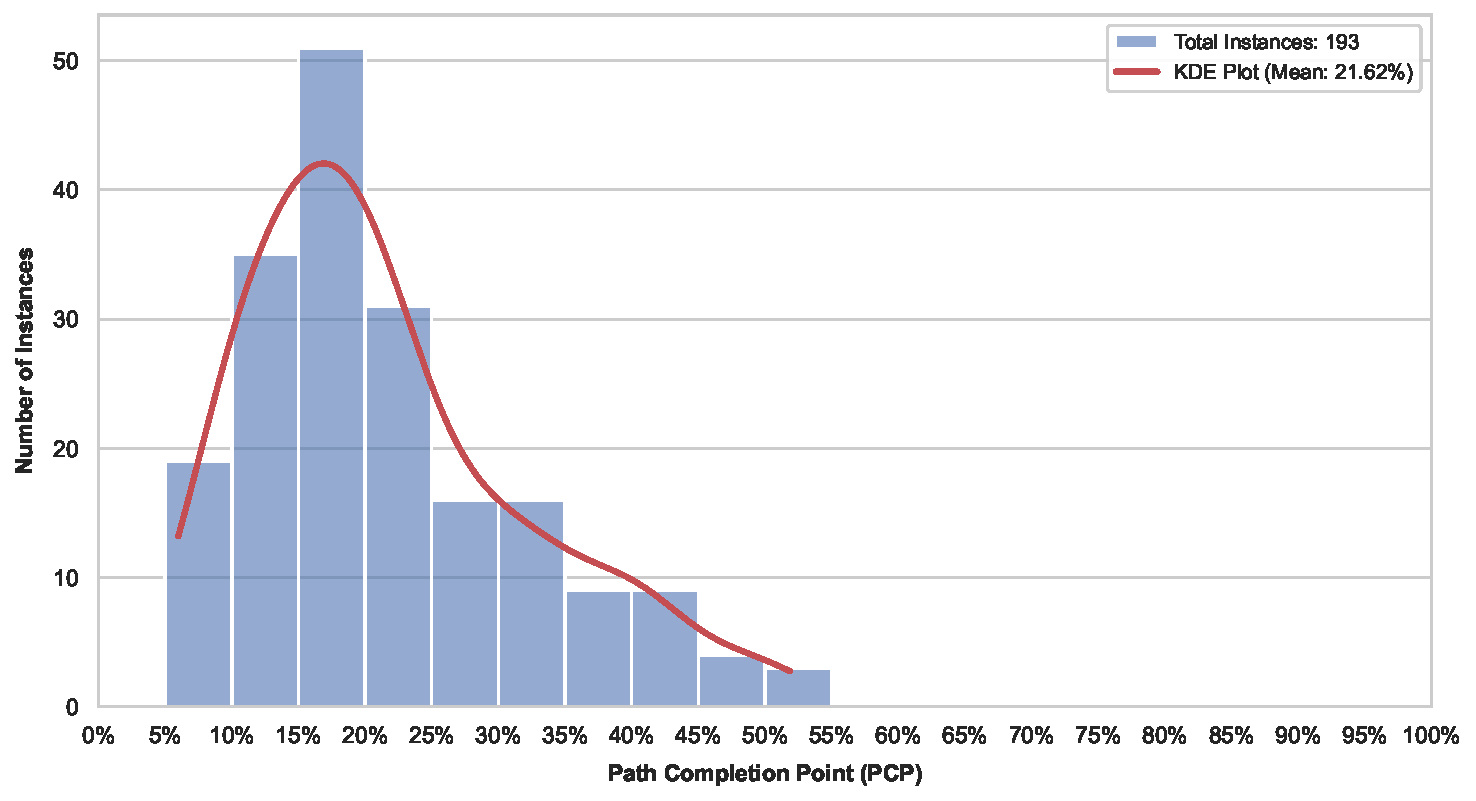
\includegraphics[width=0.9\linewidth]{figures/application/path_completion_point}
  \caption{PCP distribution for 193 instances.}
  \label{fig:path_completion_point}
\end{figure}

\figref{fig:stacked_bar_PCP} shows this behavior in more detail. The instances are grouped by their PCP. Each stacked bar shows the average number of empty, path, and class nodes. The blue line shows the ratio between path nodes and all the available space for paths:

$$\frac{\text{path nodes}}{\text{total nodes} - \text{class nodes}}$$

This ratio measures how much of the available space is occupied by paths.

As expected, this ratio increases when the PCP increases. However, we can also see that the total number of nodes decreases. This means that solutions with a higher PCP have smaller grids.

These solutions are less efficient in terms of path space. In the last groups, more than 60\% of the available space is occupied by path nodes.

\begin{figure}[ht]
  \centering
  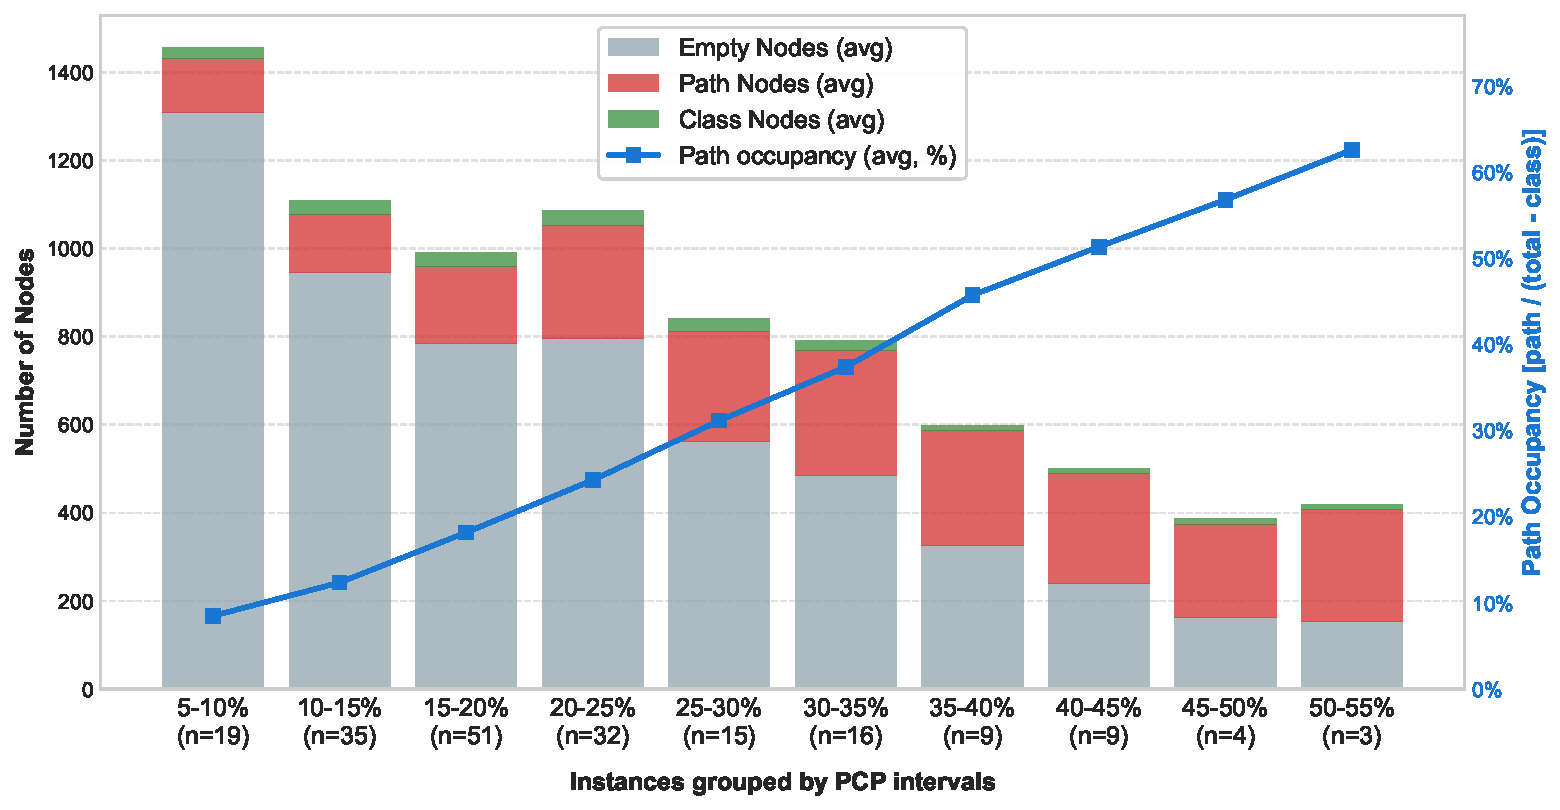
\includegraphics[width=0.9\linewidth]{figures/application/stacked_bar_PCP}
  \caption{Average node counts and path space occupancy for different PCP values.}
  \label{fig:stacked_bar_PCP}
\end{figure}

To better show this difference, \figref{fig:PCP_examples} compares four solutions generated with pure WFC. The first two solutions have the lowest PCP, 5.99\% and 7.41\%. Their paths are shorter and direct. The last two solutions have the highest PCP, 50.52\% and 50.62\%. Their paths are longer and more complex.

All four solutions are generated using pure WFC. These examples show that the PCP can also give an indication of path quality. A lower value generally corresponds to a more efficient use of the available space.

\begin{figure}[ht]
  \centering
  \resizebox{0.75\linewidth}{!}{
    \begin{minipage}{\linewidth}
      \begin{subfigure}[b]{0.48\linewidth}
        \centering
        \includegraphics[width=\linewidth]{figures/application/low_PCP_first}
        \caption{First of 193 instances, PCP = 5.99\%.}
      \end{subfigure}
      \hfill
      \begin{subfigure}[b]{0.48\linewidth}
        \centering
        \includegraphics[width=\linewidth]{figures/application/low_PCP_second}
        \caption{Second of 193 instances, PCP = 7.41\%.}
      \end{subfigure}

      \vspace{0.5em}

      \begin{subfigure}[b]{0.48\linewidth}
        \centering
        \includegraphics[width=\linewidth]{figures/application/high_PCP_penultimate}
        \caption{Next to last of 193 instances, PCP = 50.52\%.}
      \end{subfigure}
      \hfill
      \begin{subfigure}[b]{0.48\linewidth}
        \centering
        \includegraphics[width=\linewidth]{figures/application/high_PCP_last}
        \caption{Last of 193 instances, PCP = 50.62\%.}
      \end{subfigure}
    \end{minipage}
  }
  \caption{Examples of solutions with low and high PCP values.}
  \label{fig:PCP_examples}
\end{figure}

% \begin{figure}[ht]
%   \centering
  
%   \begin{subfigure}[b]{0.48\linewidth}
%     \centering
%     \includegraphics[width=\linewidth]{figures/application/low_PCP_first}
%     \caption{First of 193 instances, PCP = 5.99\%.}
%     \label{fig:low_PCP_first}
%   \end{subfigure}
%   \hfill
%   \begin{subfigure}[b]{0.48\linewidth}
%     \centering
%     \includegraphics[width=\linewidth]{figures/application/low_PCP_second}
%     \caption{Second of 193 instances, PCP = 7.41\%.}
%     \label{fig:low_PCP_second}
%   \end{subfigure}

%   \vspace{0.5em}

%   \begin{subfigure}[b]{0.48\linewidth}
%     \centering
%     \includegraphics[width=\linewidth]{figures/application/high_PCP_penultimate}
%     \caption{Next to last of 193 instances, PCP = 50.52\%.}
%     \label{fig:high_PCP_penultimate}
%   \end{subfigure}
%   \hfill
%   \begin{subfigure}[b]{0.48\linewidth}
%     \centering
%     \includegraphics[width=\linewidth]{figures/application/high_PCP_last}
%     \caption{Last of 193 instances, PCP = 50.62\%.}
%     \label{fig:high_PCP_last}
%   \end{subfigure}

%   \caption{Examples of solutions with low and high PCP values.}
%   \label{fig:PCP_examples}
% \end{figure}

\subsection{PCP vs Execution Time}

Since a lower PCP corresponds to fewer path tiles that needed to be generated, we expect that a lower PCP also leads to a shorter execution time. \figref{fig:pcp_vs_execTime_scatter} compares PCP and execution time for the 193 tested instances.

\begin{figure}[ht]
  \centering
  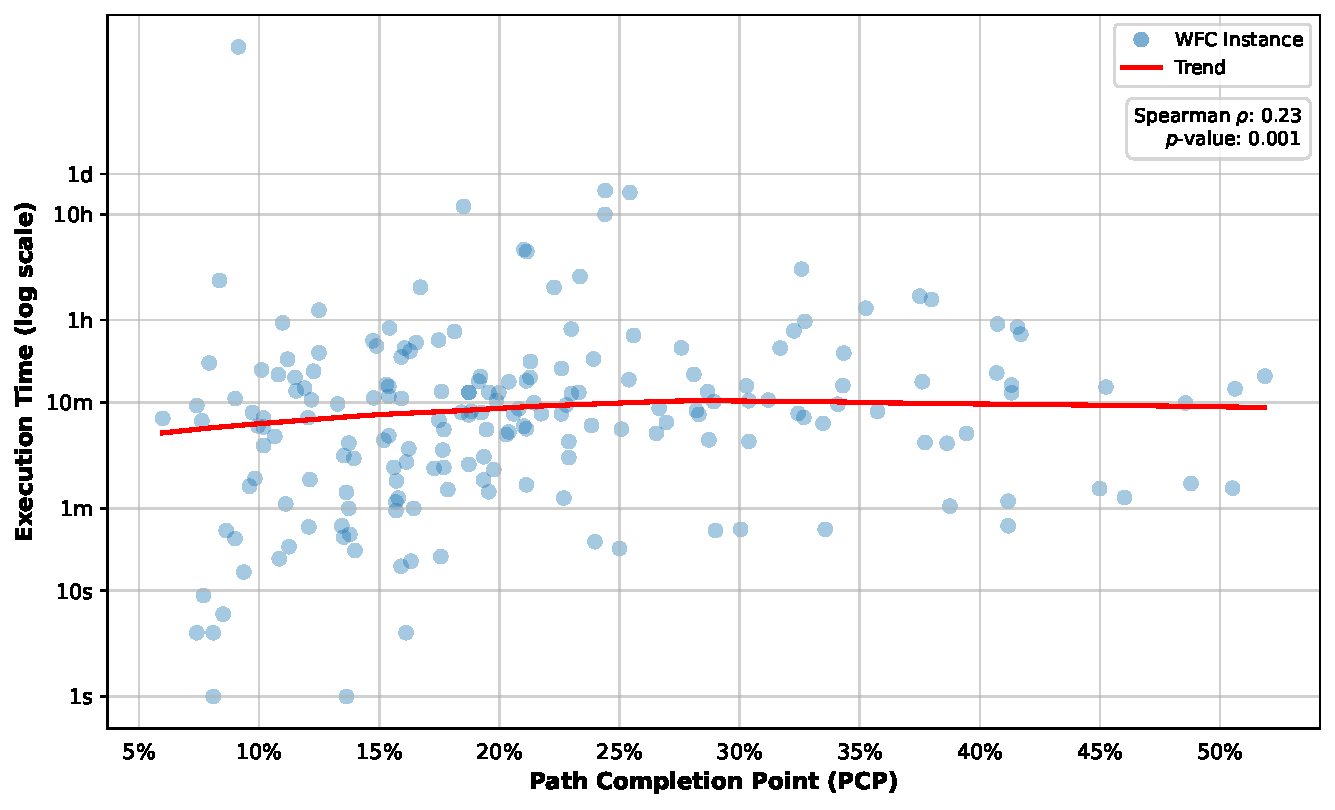
\includegraphics[width=\linewidth]{figures/application/pcp_vs_execTime_scatter}
  \caption{PCP over execution time for 193 WFC instances.}
  \label{fig:pcp_vs_execTime_scatter}
\end{figure}

As shown in the scatter plot, the points are widely scattered, showing no relationship between the two metrics. For every PCP value, the execution time varies significantly.

The absence of a clear correlation is further confirmed by the trend line, which is almost flat. The Spearman correlation is also low ($\rho = 0.23$), indicating a very weak positive correlation, although it is statistically significant ($p = 0.001$). Therefore, a lower PCP does not guarantee a faster generation time.

\end{document}